%!TEX root = SysSpec_ClockPendulumAnalyzer.tex
\subsection{Umsetzung Sensor}
\label{cap:umsetzung_sensor}
	Die Aufbau der Messvorrichtung des Sensors und dessen Anschluss ist nach folgenden Kriterien erfolgt:
	\begin{itemize}
		\item Flexible Positionierung des Sensors in der Höhe.
		\item Kleine Baugrösse um auch in kleineren Uhren messen zu können.
		\item Möglichst einfacher Anschluss mit Sicherung gegen Fehler.
	\end{itemize}
	Für den Betrieb des in Kapitel \ref{cap:sensoren} beschriebenen IR-Sensors sind im Datenblatt die in Abbildung \ref{fig:info_SFH9201} gezeigten Anschlüsse gegeben.
	\begin{figure}[H]
		\centering
		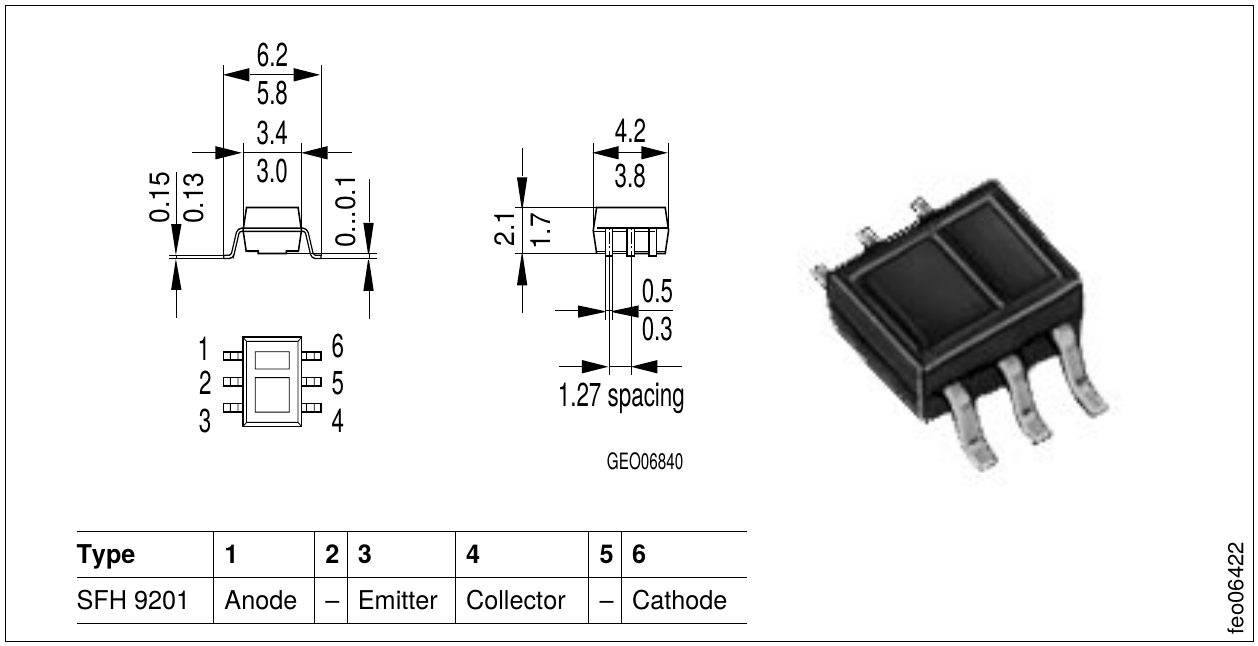
\includegraphics[width=.7\textwidth]{Sensor_layout}
		\caption{Anschlussinformationen SFH9201 (Bildquelle aus Datenblatt)}
		\label{fig:info_SFH9201}
	\end{figure}
	Weiter ist ein Schaltschema gegeben, welches den Grundaufbau der Schaltung vorgibt (Abbildung \ref{fig:schema_SFH9201}).
	\begin{figure}[H]
		\centering
		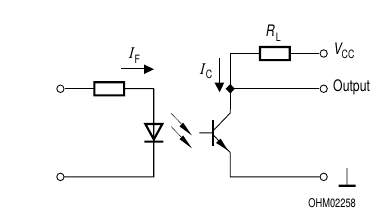
\includegraphics[width=.5\textwidth]{Sensor_Schema}
		\caption{Anschluss-Schema SFH9201 (Bildquelle aus Datenblatt)}
		\label{fig:schema_SFH9201}
	\end{figure}
	\noindent Da die Speisung der Diode und des Collectors in unserem Falle identisch sind, werden drei Anschlüsse benötigt. Eine Speisung mit 3.3V, ein Ausgang, um den Schaltzustand des Sensors zu ermitteln und ein Anschluss für Ground. 
Da es sich um einen analogen Sensor handelt, ist dem Ausgang des Sensors ein Schmitt-Trigger angehängt, welcher die Analoge Spannung in ein digitales Signal umwandelt. 
Das Verhalten des Sensors kann sich, abhängig von der Reflektion des Pendels und des Abstandes zum Pendel, verändern. Deshalb sind sowohl der Vergleichswiderstand des Schmitt-Triggers, sowie der Widerstand der Hysterese des Schmitt-Triggers mittels Potentiometer einstellbar gestaltet. 
Um die Schaltung für jedes Pendel einfach einstellen zu können, is eine grüne LED (D1) angebracht. Diese als visuelle Hilfe. Der Schaltwert ist dabei auf 3.3V, wenn kein Objekt erkannt wird und 0V, wenn ein Objekt erkannt wird. Dementsprechend verhält sich auch die LED. Gemeinsam ist das in Abbildung \ref{fig:schema_sensor} dargestellte Schema entstanden.
	\begin{figure}[H]
		\centering
		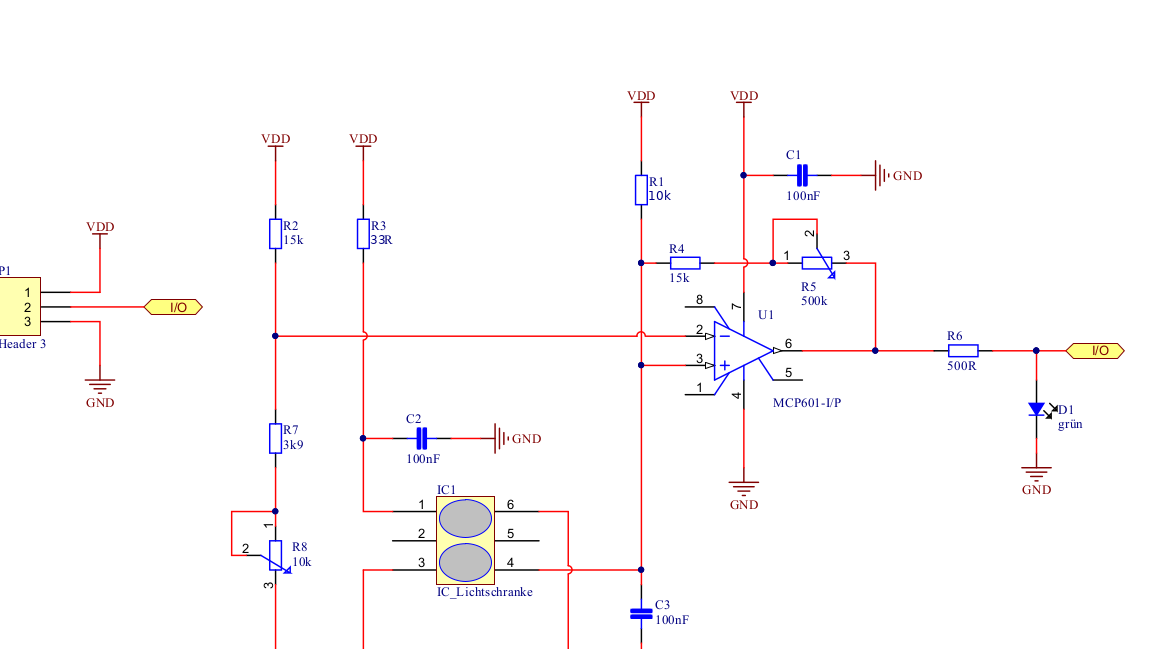
\includegraphics[width=.9\textwidth]{Circuit_Sensor}
		\caption{Ermitteltes Elektroschema für das Sensor-PCB SFH9201}
		\label{fig:schema_sensor}
	\end{figure}
	\noindent Ein falsches Anschliessen des Sensors wird durch das gewählte Steckersystem verhindert. Der Widerstand R1 mit 33$\Omega$ ist der Vorgabe gemäss Datenblatt berechnet. Diese sind:
	\begin{itemize}
		\item 1.65V als maximale und gemessene Spannung $U_{IRD}$ über der IR-Diode
		\item 50mA Betriebsstrom $I_F$
	\end{itemize}
	Ausgehend von einer Speisung $U_S$ von 3.3V ergibt dies folgende Formel:
	\[
		R = \frac{U_S - U_{IRD}}{I_R} = \frac{3.3 - 1.65}{0.05} = 33\Omega
	\]
	Die Werte für die Potentiometer wurden in Zusammenarbeit mit der Elektrotechnik ermittelt. Der 3.9$k\Omega$ Widerstand R7 dient als Minimalwiderstand für die Schwellspannung, welche mit dem Potentiometer R8 justiert werden kann. Diese Einstellung entscheidet, bei wie viel Reflektion ein Pendel registriert wird.
Das Potentiometer R5 dient zum Einstellen, bei welcher Spannung zurückgeschaltet wird um ein Flattern zu vermeiden.
Ein entsprechendes PCB\footnote{Printed Circuit Board} ist an der Hochschule Luzern, Technik \& Archtektur erstellt worden (Abbildung \ref{fig:Sensor_overview}).\\
	\begin{figure}[H]
		\centering
		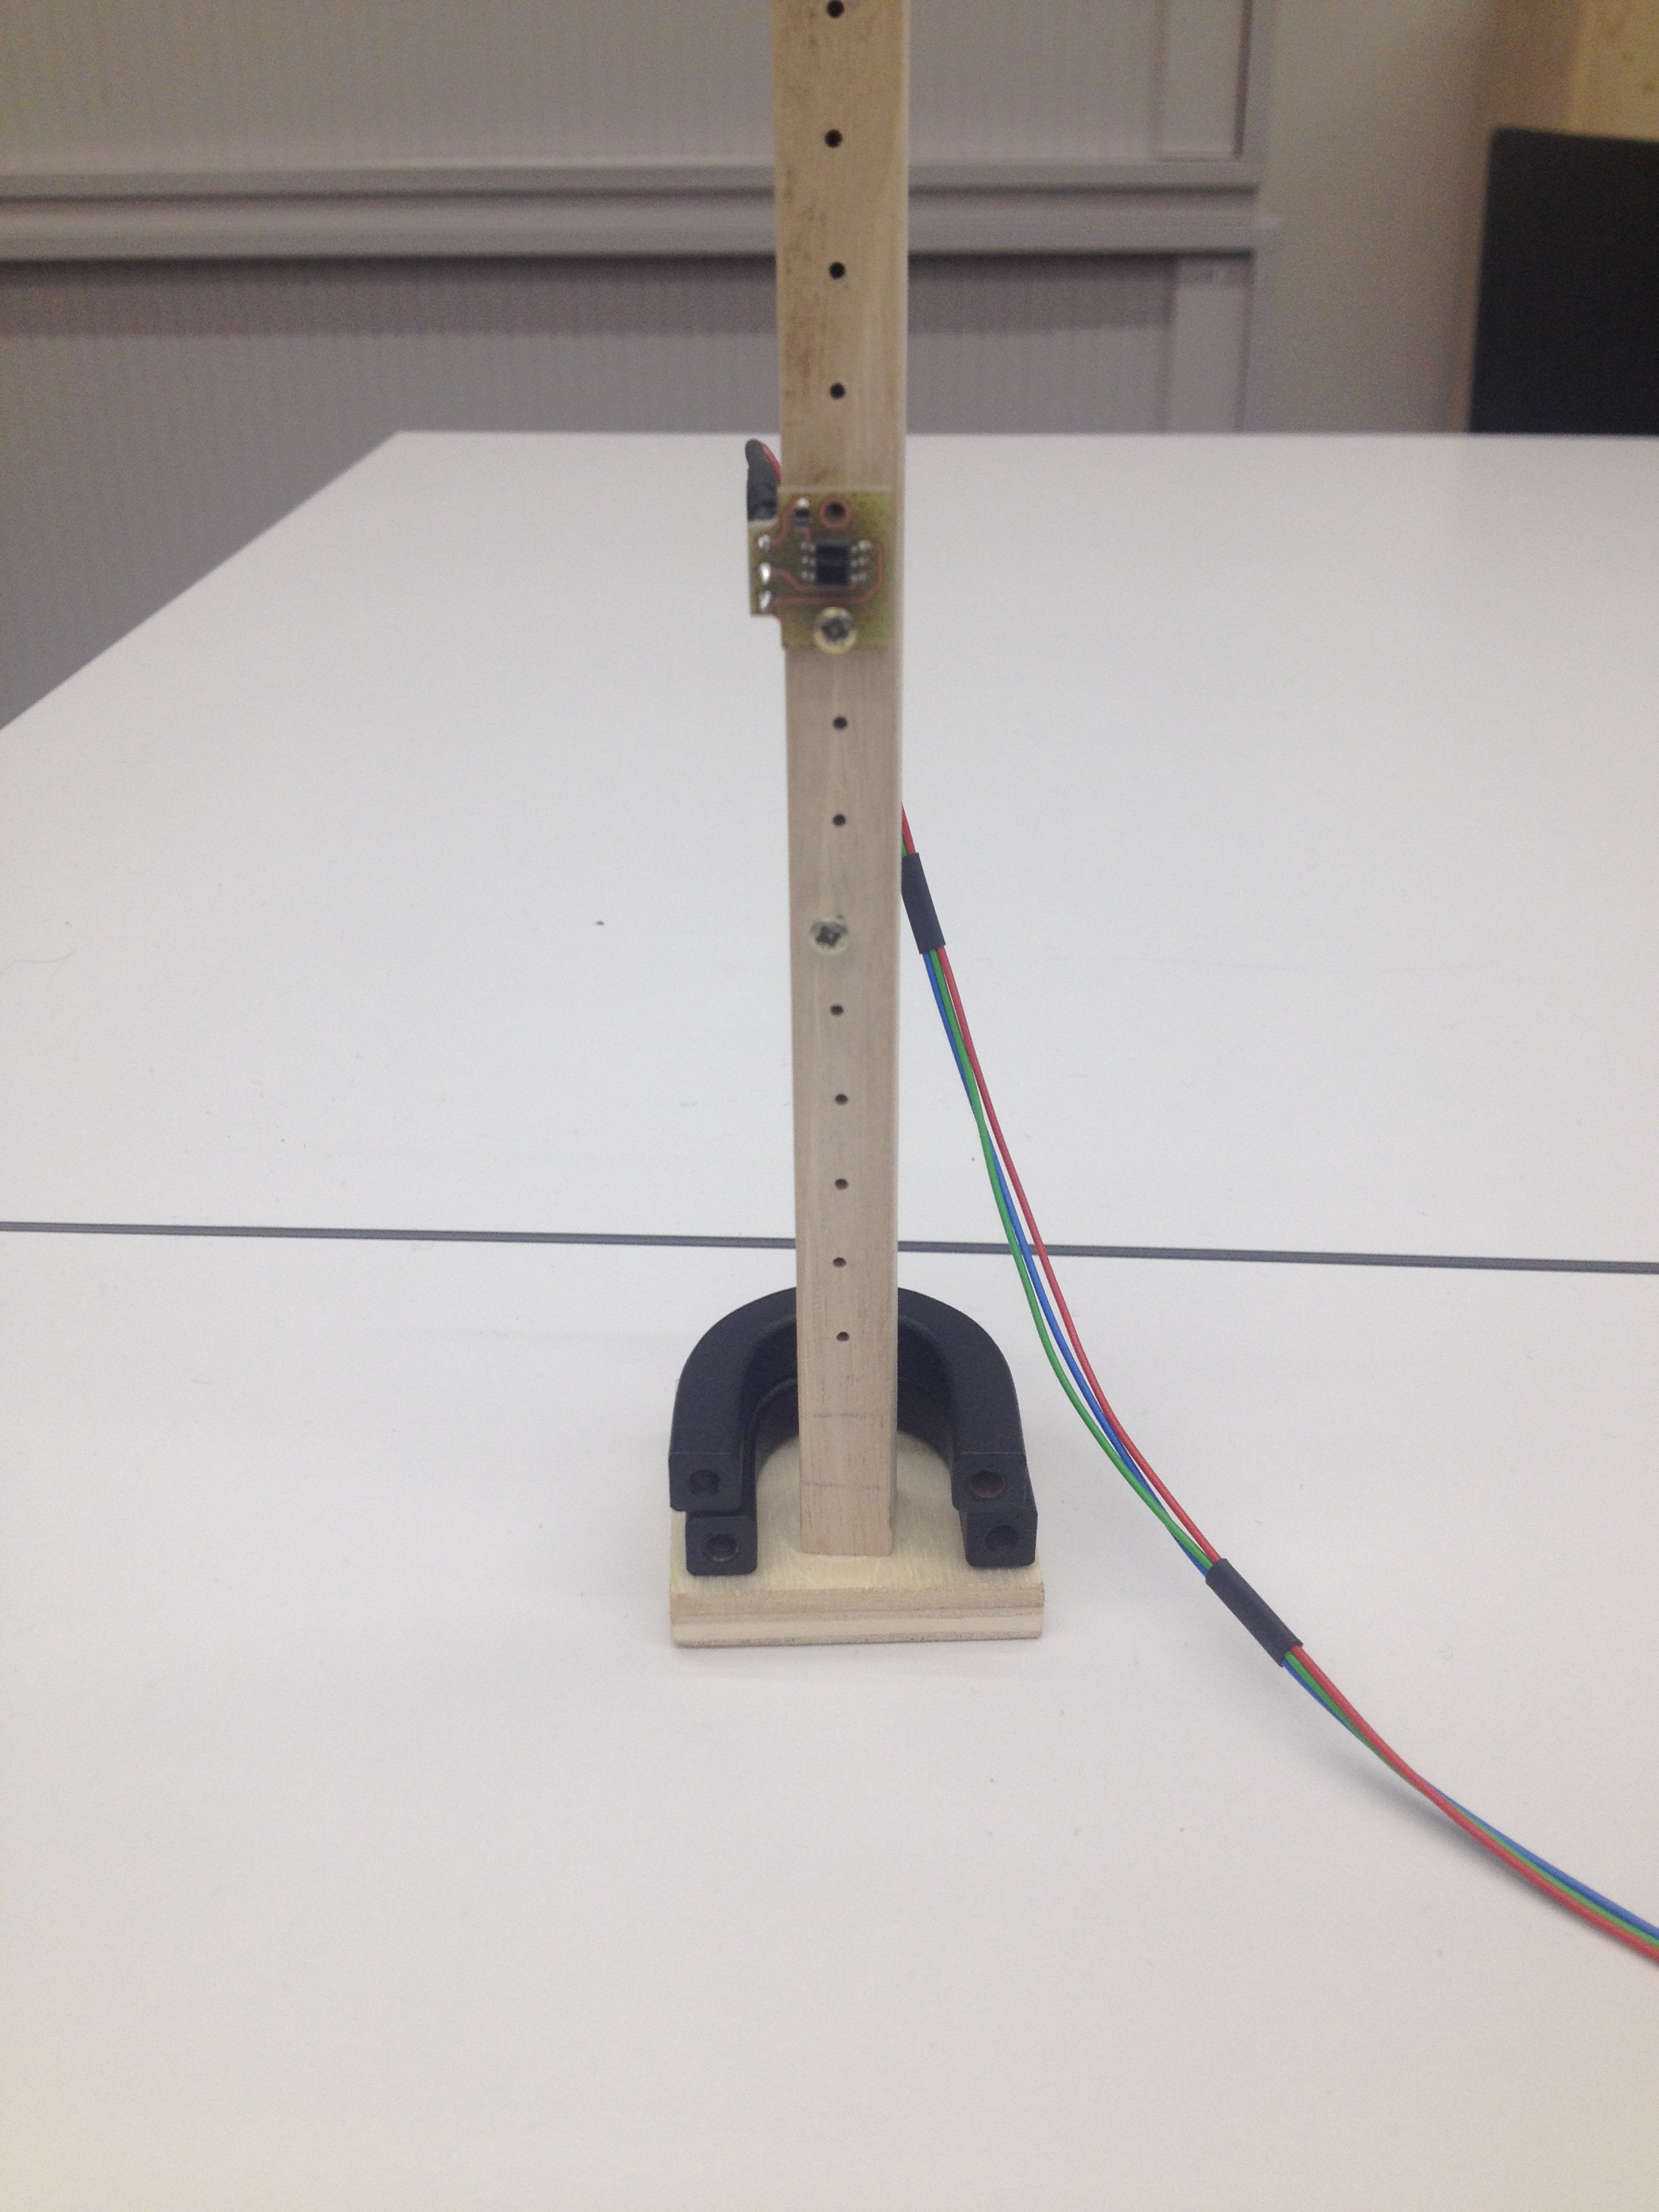
\includegraphics[width=.4\textwidth]{Sensor_overview}
		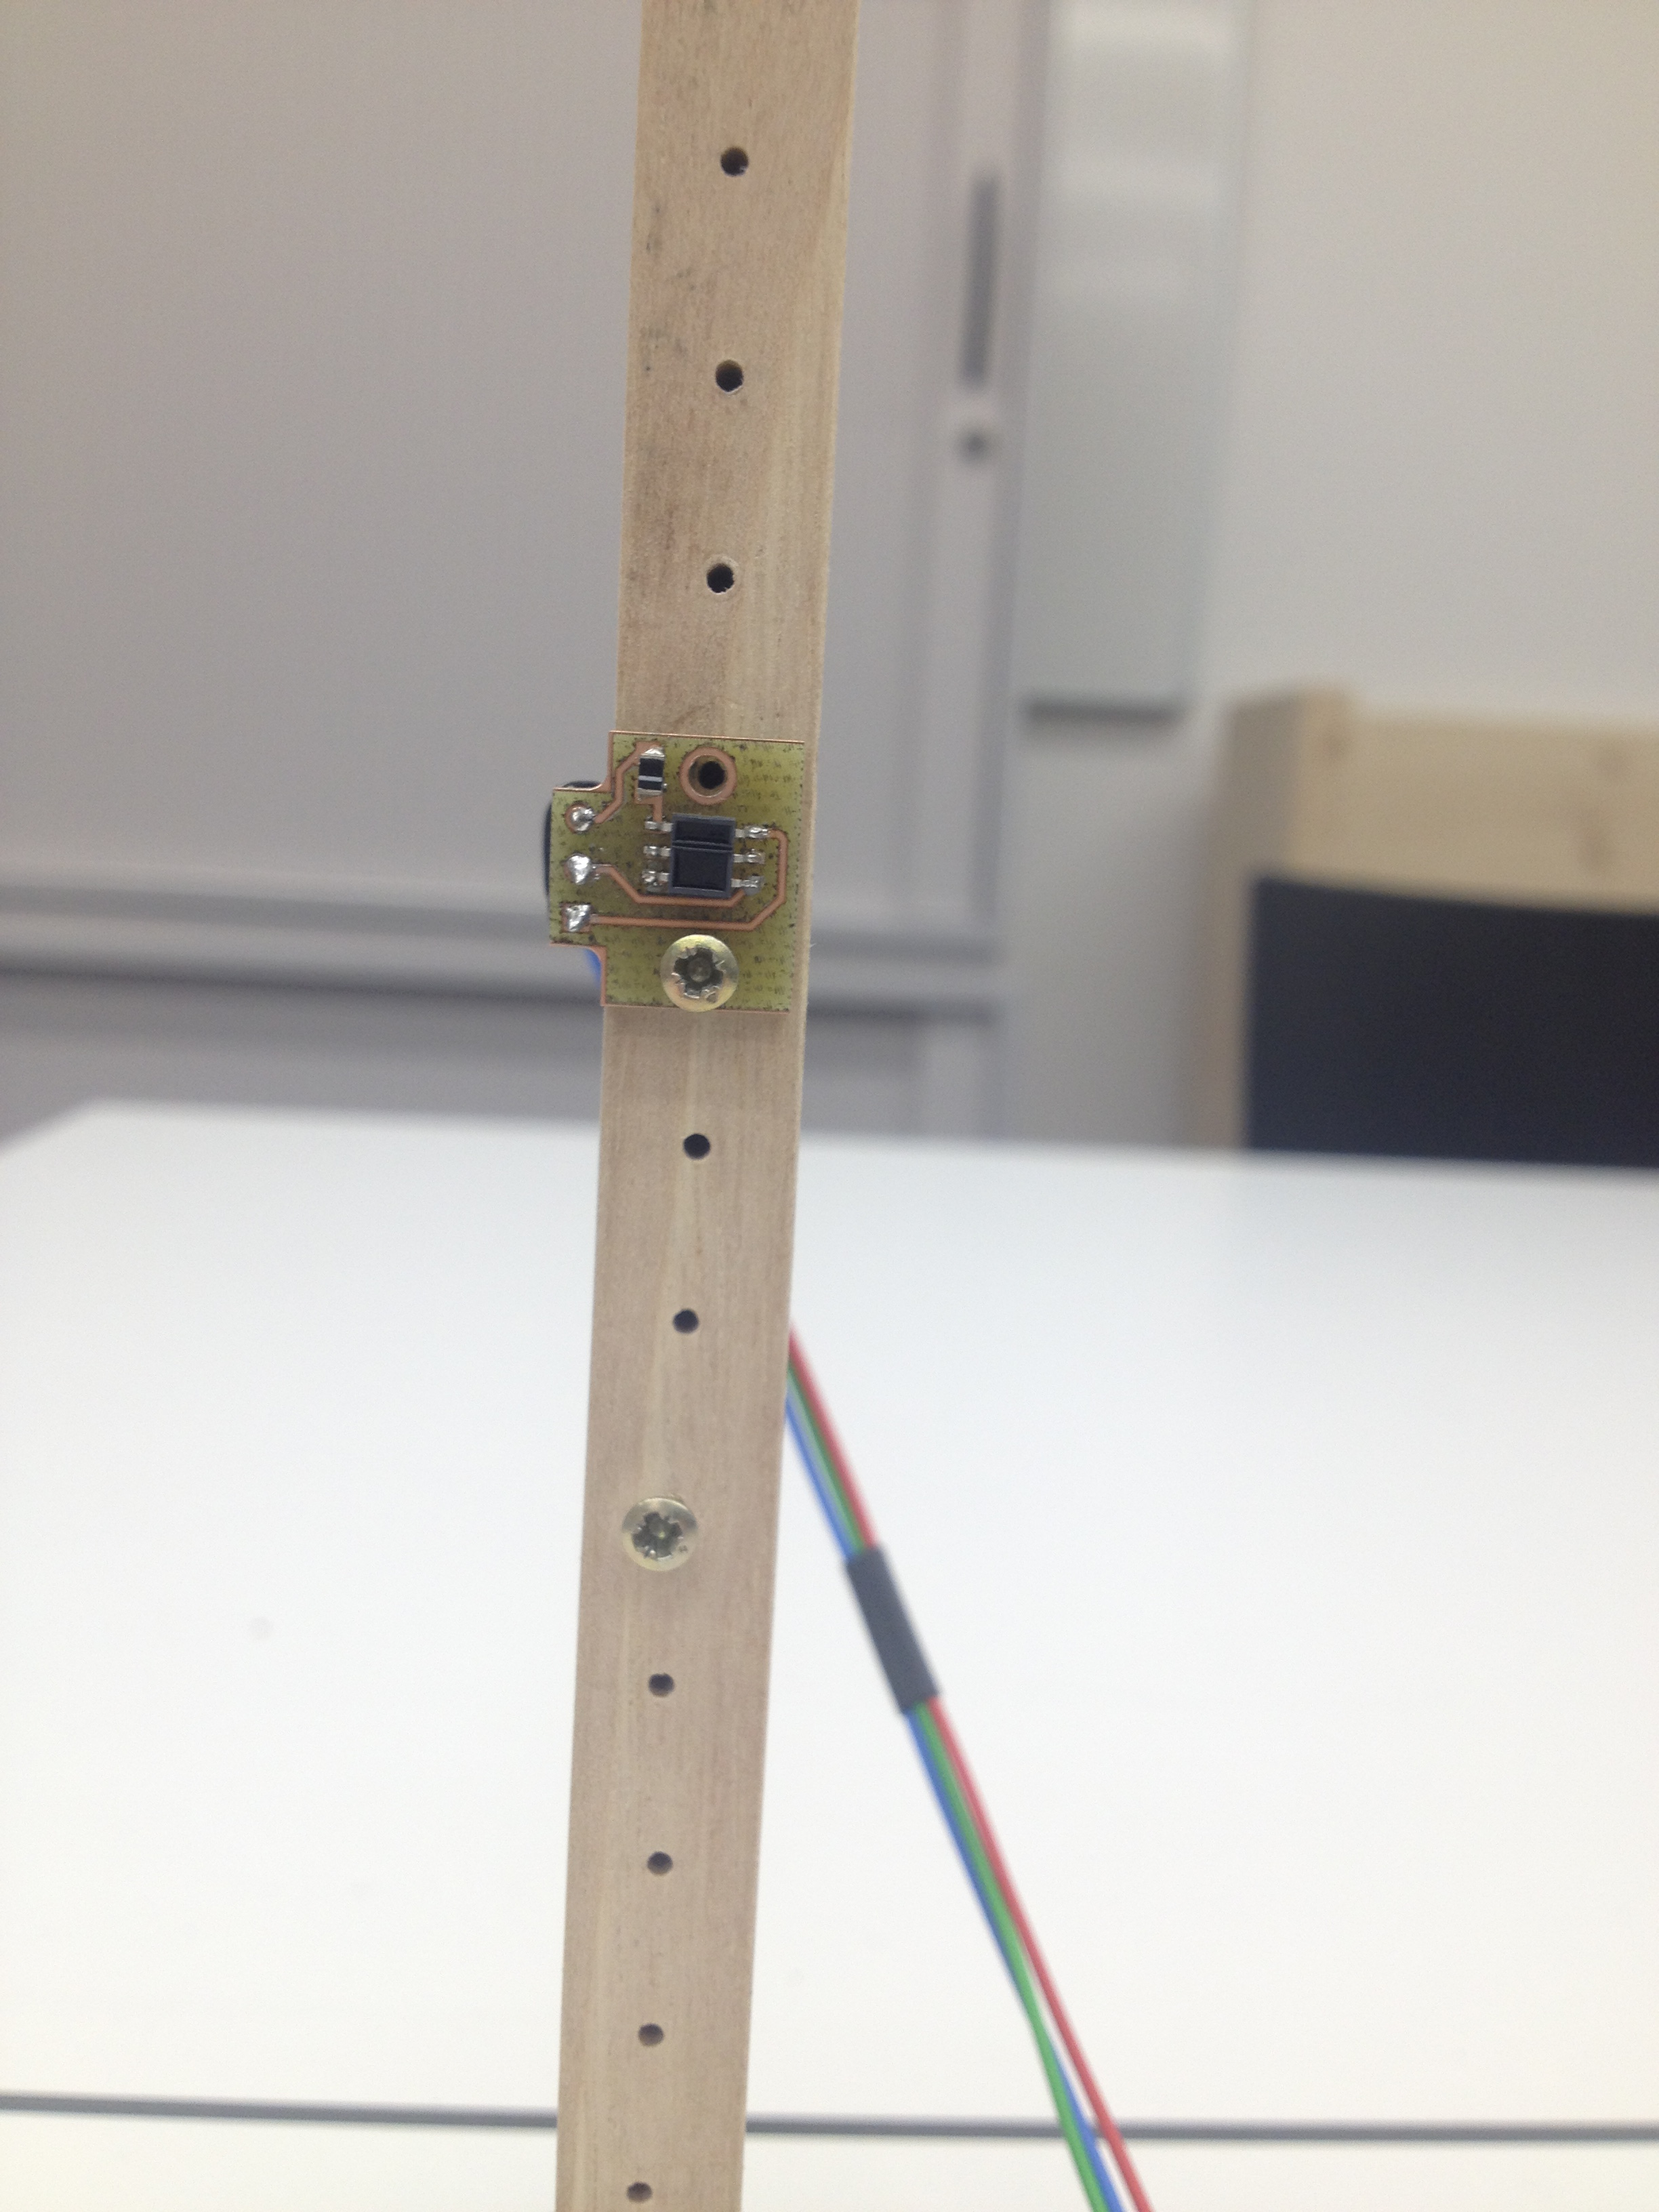
\includegraphics[width=.4\textwidth]{Sensor_Detail}
		\caption{Aufbau des Sensors für die Pendelmessung}
		\label{fig:Sensor_overview}
	\end{figure}
	\noindent Als Stütze für den Sensor dient eine Holzkonstruktion, welche über ein Lochraster von 10mm verfügt, an welchen sich der Sensor befestigen lässt. So können verschiedene Pendellängen und Anordungen abgedeckt werden (Abbildung \ref{fig:Sensor_FullView}). Zwei Gewichte am Fuss verhindern ein Kippen der Konstruktion.
	\begin{figure}[H]
		\centering
		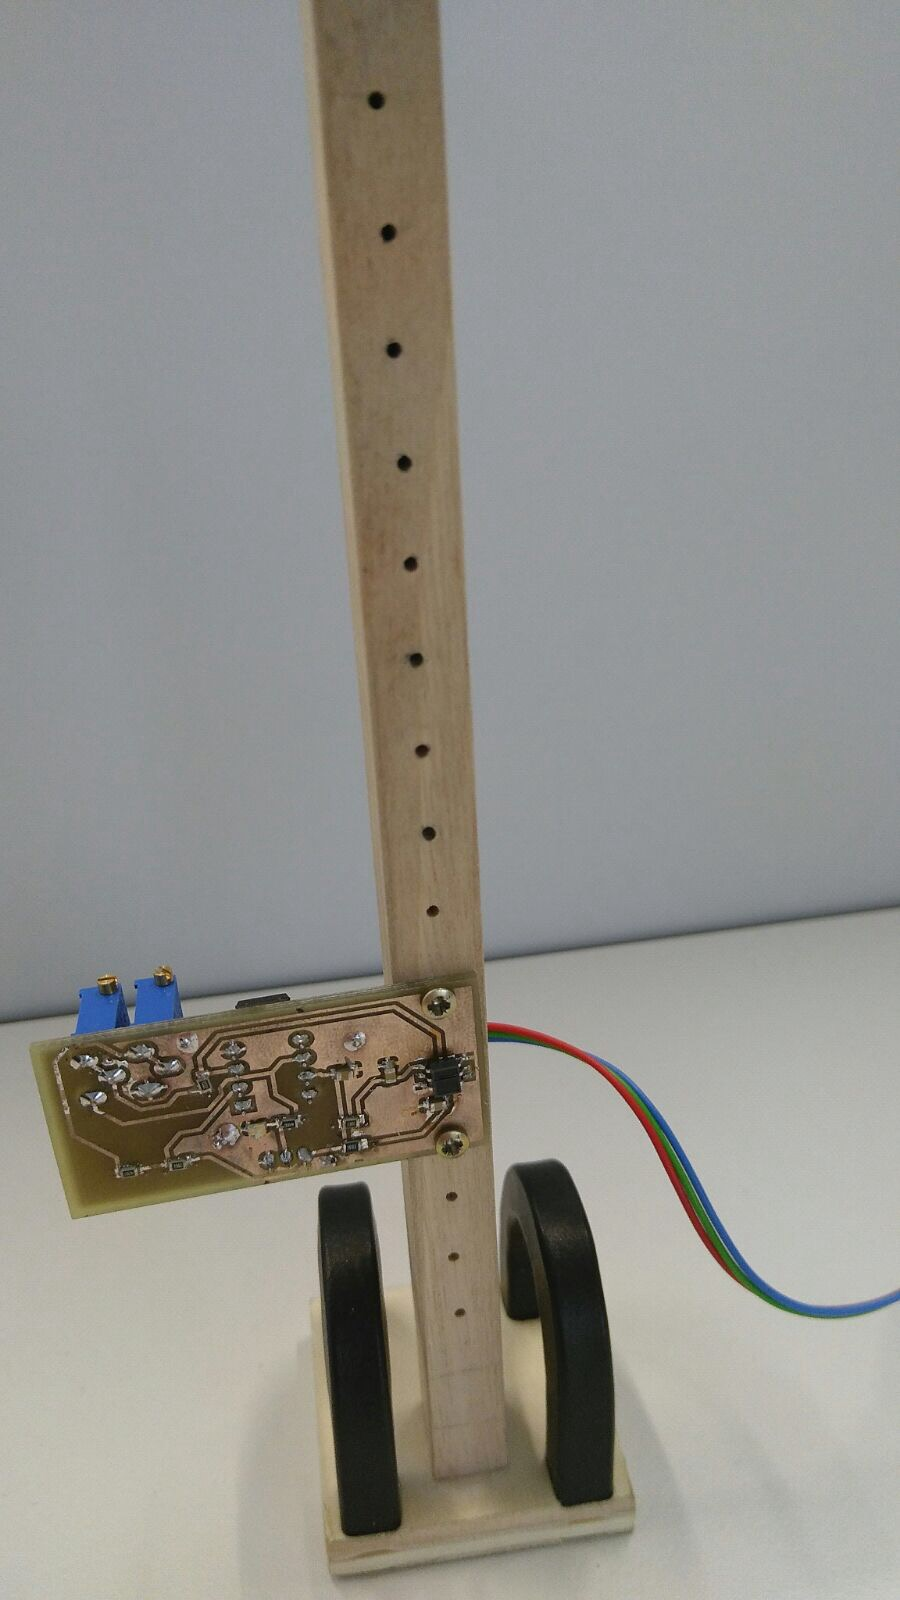
\includegraphics[width=.25\textwidth]{Sensor_FullView}
		\caption{Aufbau des Sensors für die Pendelmessung}
		\label{fig:Sensor_FullView}
	\end{figure}
	\noindent Der Sensor sollte für ein optimales Ergebnis maximal 5mm vom nächsten Punkt am Pendel entfernt angebracht werden. Weiter sollte das Pendel möglichst mittig erfasst werden, um Streuungen zu vermeiden. Die zuvor beschriebene LED (D1 in Abbildung \ref{fig:Sensor_overview} muss konstant aus sein, wenn sich das Pendel vor dem Sensor befindet. 
Der Sensor lässt sich entweder am Rand der Bahn anbringen, dann wird jede Messung erfasst und das Pendel passiert den Sensor nicht vollständig oder mittig, wenn das Pendel den Sensor vollständig passieren soll. Im zweiten Fall muss dann jede zweite Messung verworfen werden, damit das Pendel immer von der selben Seite erfasst wird. Abbildung \ref{fig:sensor_position} zeigt einen optimalen Positionierbereich für den Sensor, innerhalb des roten Rahmens.
	\begin{figure}[H]
		\centering
		\includegraphics[width=.25\textwidth]{sensor_position}
		\caption{Optimale Position des Sensors für die Pendelmessung}
		\label{fig:sensor_position}
	\end{figure}